% ---------------------------------------------------------------- Appendix C
\clearpage
\section{Additional results}\label{app:C}

\begin{table}[htbp]\centering\footnotesize
\caption{Market-priced debt in the two-state model}\label{tab:C1}
\begin{tabularx}{\linewidth}{@{}l*{4}{C}@{}}
\toprule
$D$ & $\VL - \VU$, fixed rate & Lenders' loss, fixed rate & $\VL - \VU$, market-priced & Break-even rate \\
\midrule
40 & 0.73    & 0.00  & 0.73    & 10.0\% \\
44 & 0.80    & 0.00  & 0.80    & 10.0\% \\
45 & $-3.63$ & 4.72  & $-2.16$ & 29.9\% \\
50 & $-3.55$ & 7.18  & $-1.32$ & 37.2\% \\
55 & $-3.46$ & 9.65  & $-0.47$ & 43.3\% \\
60 & $-3.38$ & 12.11 & 0.38    & 48.3\% \\
\bottomrule
\end{tabularx}
\tablenote{\textit{Notes:} Beyond the debt limit only the strong state services the debt, so the promised coupon rises sharply; because that coupon is deductible in the strong state, market pricing moderates the fall in value. This is an artefact of the two-state model; in the lognormal model (Table~\ref{tab:C2}) the two pricing rules give similar firm values up to $D = 50$.}
\end{table}

\begin{table}[htbp]\centering\footnotesize
\caption{Market-priced debt in the lognormal model}\label{tab:C2}
\begin{tabularx}{\linewidth}{@{}l*{6}{C}@{}}
\toprule
$D$ & $\VL - \VU$, fixed & P(default), fixed & Shareholders' gain, fixed & $\VL - \VU$, market & Break-even rate & P(default), market \\
\midrule
20 & 0.36    & 0.0\%  & 0.36 & 0.36    & 10.0\% & 0.0\%  \\
30 & 0.53    & 0.3\%  & 0.55 & 0.53    & 10.1\% & 0.3\%  \\
34 & 0.56    & 1.0\%  & 0.65 & 0.57    & 10.3\% & 1.0\%  \\
35 & 0.55    & 1.3\%  & 0.68 & 0.57    & 10.4\% & 1.4\%  \\
40 & 0.43    & 4.1\%  & 0.89 & 0.51    & 11.4\% & 4.4\%  \\
45 & 0.05    & 9.6\%  & 1.31 & 0.19    & 13.8\% & 11.5\% \\
50 & $-0.66$ & 18.0\% & 2.06 & $-0.58$ & 19.3\% & 25.0\% \\
55 & $-1.68$ & 28.5\% & 3.29 & $-2.19$ & 32.5\% & 49.9\% \\
\bottomrule
\end{tabularx}
\tablenote{\textit{Notes:} 200,000 draws, lognormal EBIT with mean 90 and standard deviation 25.}
\end{table}

\begin{figure}[htbp]\centering
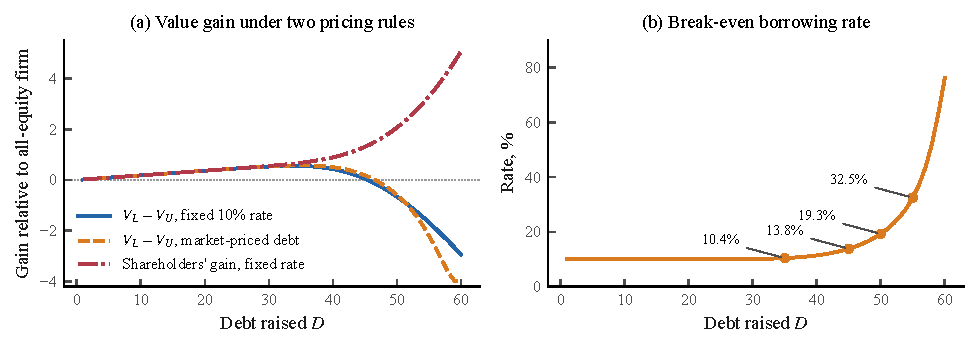
\includegraphics[width=14.2cm]{figC1_market_debt}
\caption{Market-priced debt in the lognormal model. (a) Value gain under fixed-rate and break-even pricing, and the gain perceived by shareholders under a fixed rate. (b) Borrowing rate at which lenders break even.}\label{fig:C1}
\end{figure}

\begin{table}[!htbp]\centering\footnotesize
\caption{Usable share of the statutory tax shield (\%), by interest coverage}\label{tab:C3}
\begin{tabularx}{\linewidth}{@{}l*{7}{C}@{}}
\toprule
EBIT volatility & 1  & 1.5 & 2  & 3   & 3.33 & 5   & 10  \\
\midrule
0.28            & 89 & 98  & 99 & 100 & 100  & 100 & 100 \\
0.28 + cap      & 30 & 45  & 60 & 84  & 89   & 98  & 100 \\
0.60            & 77 & 86  & 89 & 92  & 92   & 93  & 94  \\
0.60 + cap      & 30 & 45  & 58 & 74  & 77   & 86  & 92  \\
1.00            & 68 & 74  & 77 & 80  & 80   & 82  & 83  \\
1.00 + cap      & 32 & 46  & 56 & 66  & 68   & 74  & 80  \\
\bottomrule
\end{tabularx}
\tablenote{\textit{Notes:} No loss carry-forward; ``+ cap'' adds a 30\%-of-EBIT limit on deductible interest. Normal EBIT, 300,000 draws.}
\end{table}

\begin{table}[htbp]\centering\footnotesize
\caption{Present value of the shield on $D = 40$ maintained for $T$ years ($\tauc = 20\%$, $r = 10\%$)}\label{tab:C4}
\begin{tabularx}{\linewidth}{@{}l*{5}{C}@{}}
\toprule
$T$ (years)  & 1    & 5    & 10   & 30   & Perpetual \\
\midrule
PV of shield & 0.73 & 3.03 & 4.92 & 7.54 & 8.00      \\
\bottomrule
\end{tabularx}
\end{table}
